\documentclass[a4paper,12pt]{article}
\usepackage{amsmath}
\usepackage{amssymb}
\usepackage{graphicx}
%\documentclass{article}
\usepackage{setspace, enumitem,titlesec}
\usepackage{calc}
			% Activate to display a given date or no date
\usepackage{mathtools}
\usepackage{mathrsfs }
\DeclarePairedDelimiter\ceil{\lceil}{\rceil}
\DeclarePairedDelimiter\floor{\lfloor}{\rfloor}
\usepackage{algorithm}
\usepackage{algorithmic}
\usepackage{fancybox}

\usepackage{amsmath}
\usepackage{amssymb}
\usepackage{amsthm}
%\usepackage{algpseudocode}
\begin{document}
%\renewcommand{\thepseudonum}{\roman{pseudonum}}
\renewcommand\labelenumi{(\theenumi)}
%vector
\renewcommand{\vec}[1]{\mathbf{#1}}
\title {From law of large number to the culture computation }
%\author{jim.morris.shen@gmail.com}
%\author{The Graduate Center, City University of New York}
\author{Xiaoke(Jimmy) Shen}
\maketitle
%\textbf{Due Mar 1st 11:59 pm. 10 points for each exercise and 20 points for the extra credit exercise }\\
\section{Introduction}
Culture is important to everyone. Better understanding a culture can help the people with different background and culture know each other in a better way. How to do the culture mining or computation? Thanks for the theory from mathematics and also thanks to the modern computer technologies, it seems we do can find some ways to explore the culture by doing the data analysis, such find the sleeping time of a city.\\
\section{Law of Large Number}
Law of large number is one of the most wonderful law in this world(another one is  from my personal's point of view). It shows us that after we get enough repeat observation or sampling , we can have some insight about the object we are observing. The theory will not be proved here as I am not from mathematics department. However, the simulation will be done here to demo the basic idea about the law of large number.\\
\begin{figure}[H]
  \begin{center}
      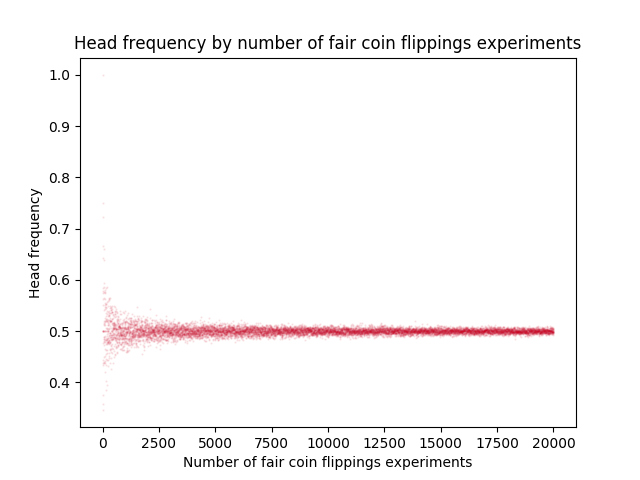
\includegraphics[scale=0.8]{law_of_large_number.png}
\end{center}
\caption{An illustration of the law of large numbers by using a fair coin to do the flipping experiments.}
 \label {fig:2}
 \end{figure}
The illustration of the law of large numbers using a fair coin to do the flipping experiments. As the number of experiments increases, the average of getting the head ratio of all the results approaches to 0.5.\\

\section{What is the sleeping time for a city?}
Since the law of large number tells us with enough observations, we can get some stable observations. I am going to do something based on this law to see whether we can exploring the sleeping time of 5 cities(The data is provided by the Cultural Analytics Lab of the Graduate Center, CUNY). Those five cities are Buenos Aires, London, Los Angeles, Nairobi and Tokyo.\\
  \begin{figure}[H]
  \begin{center}
      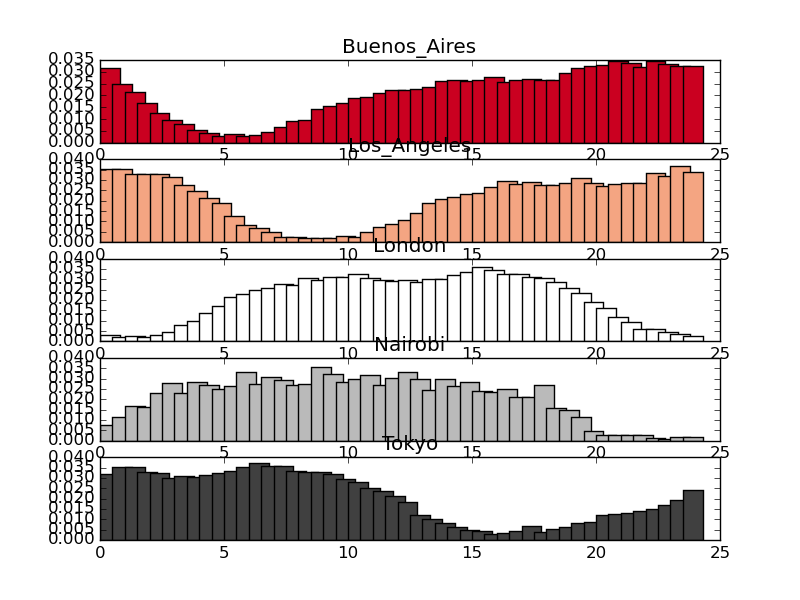
\includegraphics[scale=0.8]{final.png}
\end{center}
\caption{Final result of the sleeping time analysis of 5 cities. The x axis shows the time period of a day from 0:00 am to 23:59 pm. And each period is 30 minutes. The y axis is the activation ratio of the specified time period.}
 \label {fig:2}
 \end{figure}
The final result is shown in figure 2.  The x axis shows the time period of a day from 0:00 am to 23:59 pm. And each period is 30 minutes. The y axis is the activation ratio of the specified time period. From the result we can see different cities has totally different work and rest style. If we take the small value of activation ratio as the sleeping time of the city, each city has different sleeping time which strongly related to the life style and culture.\\

How can we get it? Following sessions are the step by step explanation to show how finally we find some insight about the sleeping time of a city.\\

\subsection{Observe the twitter post every minute}
If we observe the twitter post every minute, the visualization results are shown in the following figures. From the histogram of the 5 cities twitter post per minute we can see this value is mainly between 0 and 10.  The twitter post number per minute for each city is visualized by using a gray leve image. When we get a pure dark point, it means that point has the maximum number of the twitter post. When the gray level is smaller, then it means the number of post is decreased. When there is no post, it will become 0 which is totally blank.  In the data argumentation part, a threshold is set to make sure the result only has two status 0 and 1 to help us find a better insight behind the data.\\

From those result we already see some structure of the active level for each city based on time slots. \\




\begin{figure}[H]
  \begin{center}
      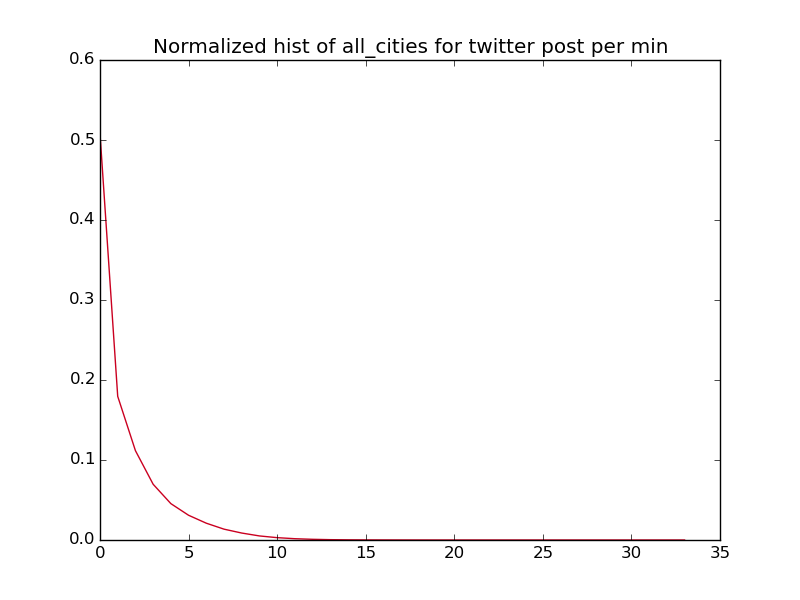
\includegraphics[scale=0.8]{all_citieshisto.png}
\end{center}
\caption{Histogram of five cities when the observation time slot is every one minute}
 \label {fig:2}
 \end{figure}



\begin{figure}[H]
  \begin{center}
      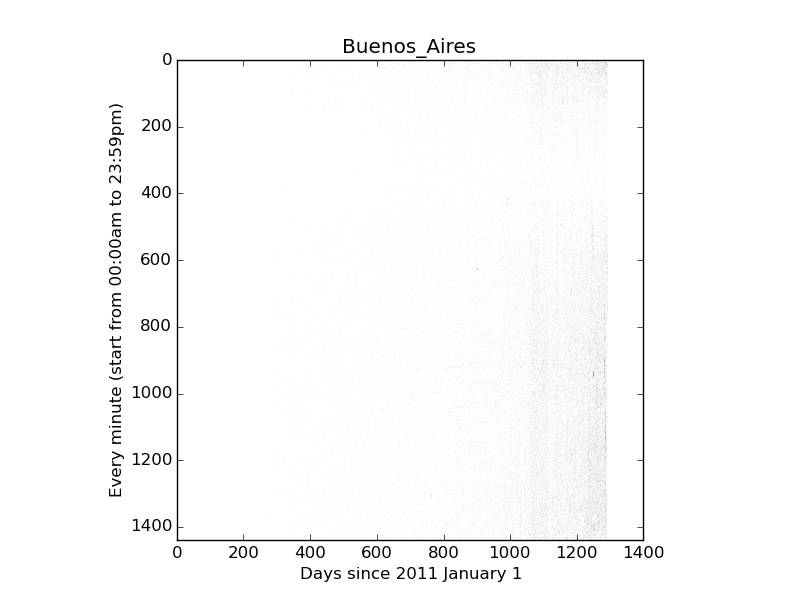
\includegraphics[scale=0.8]{Buenos_Aires.png}
\end{center}
\caption{Buenos Aires every minute without data argumentation}
 \label {fig:2}
 \end{figure}



\begin{figure}[H]
  \begin{center}
      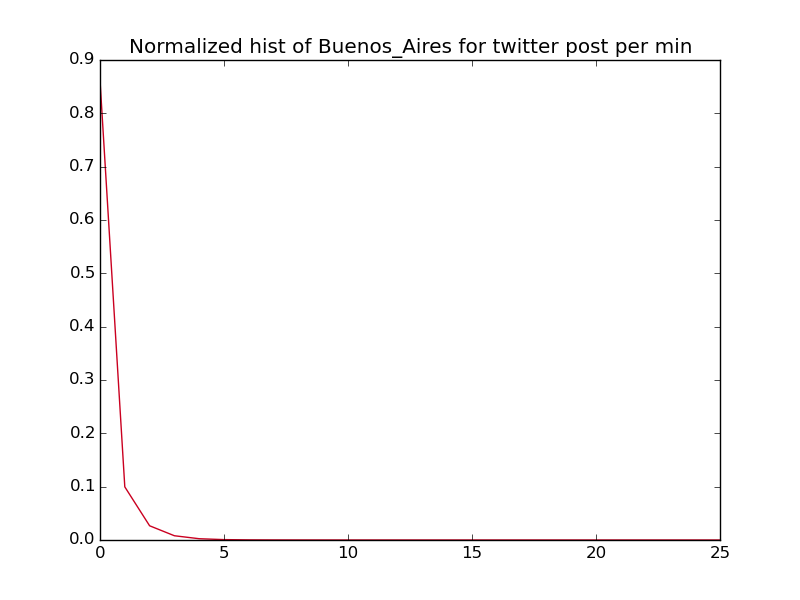
\includegraphics[scale=0.8]{Buenos_Aireshisto.png}
\end{center}
\caption{Histogram of Buenos Aires}
 \label {fig:2}
 \end{figure}


\begin{figure}[H]
  \begin{center}
      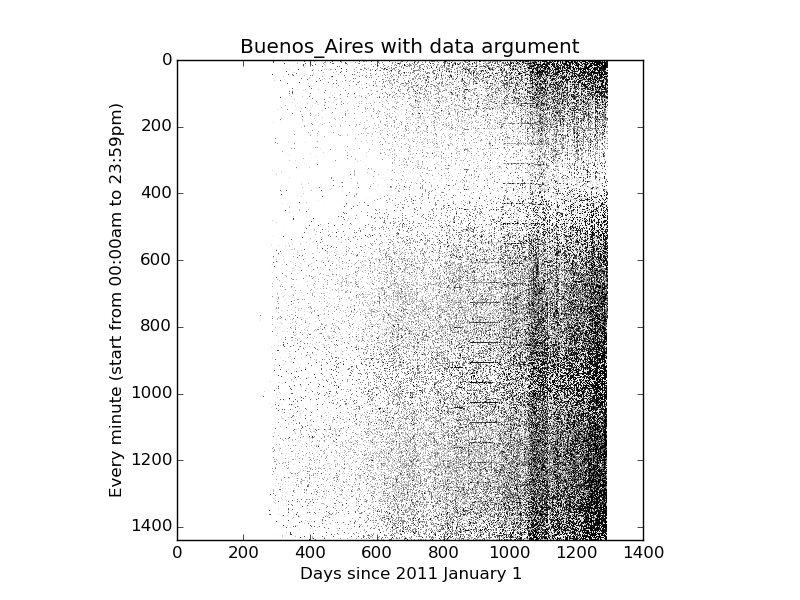
\includegraphics[scale=0.8]{Buenos_Airesbinary.png}
\end{center}
\caption{Buenos Aires every minute with data argumentation}
 \label {fig:2}
 \end{figure}










\begin{figure}[H]
  \begin{center}
      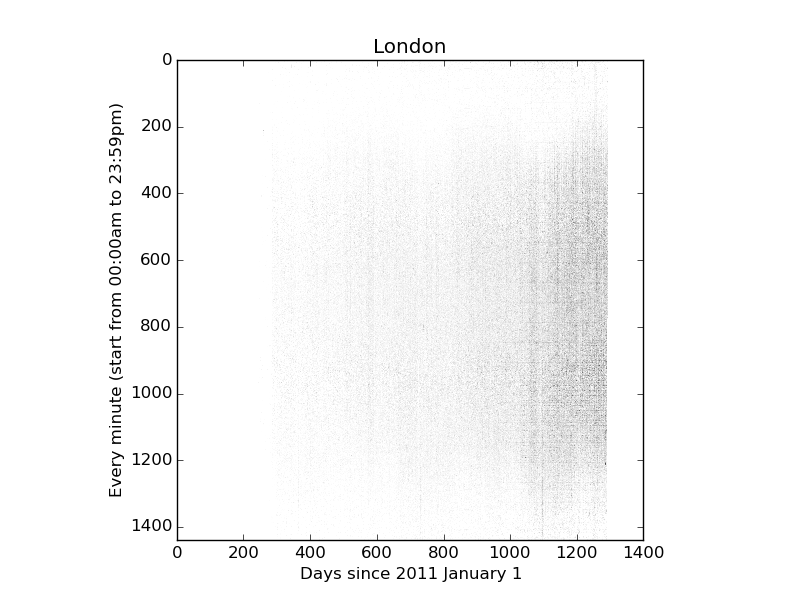
\includegraphics[scale=0.8]{London.png}
\end{center}
\caption{London every minute without data argumentation}
 \label {fig:2}
 \end{figure}

\begin{figure}[H]
  \begin{center}
      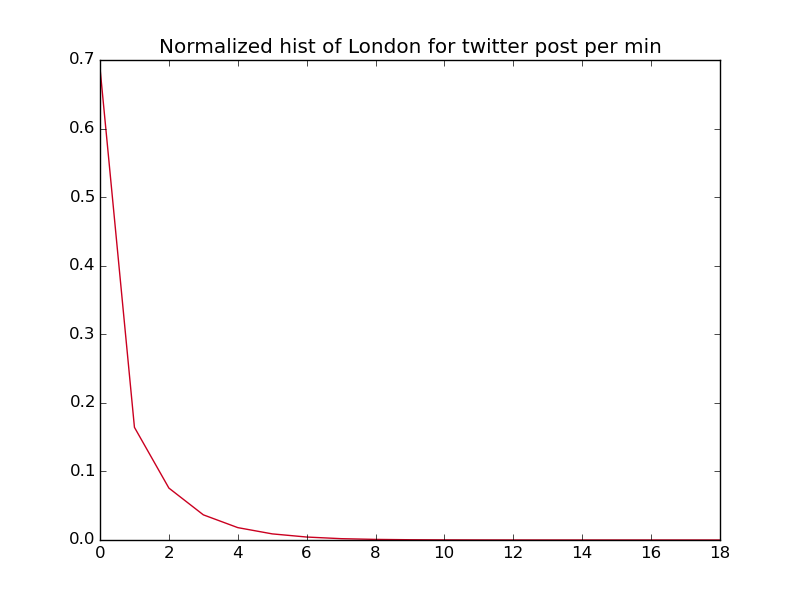
\includegraphics[scale=0.8]{Londonhisto.png}
\end{center}
\caption{Histogram of London}
 \label {fig:2}
 \end{figure}

\begin{figure}[H]
  \begin{center}
      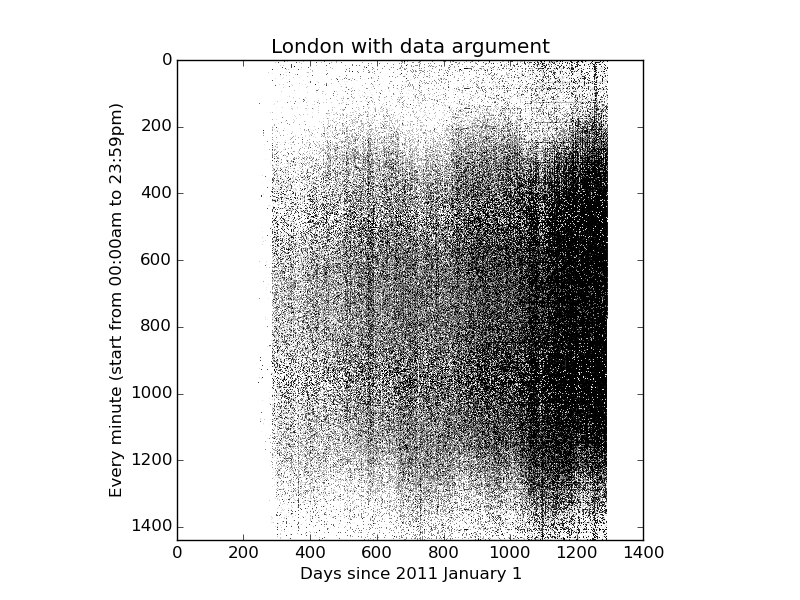
\includegraphics[scale=0.8]{Londonbinary.png}
\end{center}
\caption{London every minute with data argumentation}
 \label {fig:2}
 \end{figure}






\begin{figure}[H]
  \begin{center}
      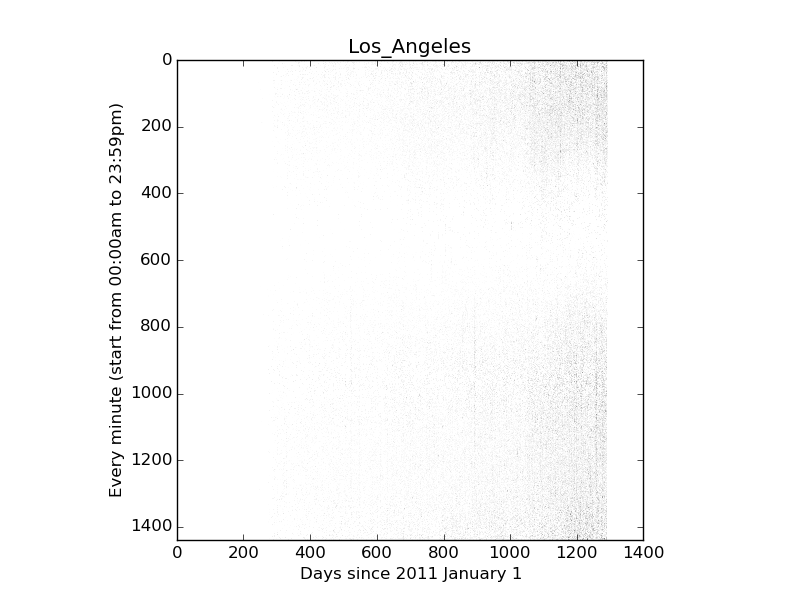
\includegraphics[scale=0.8]{Los_Angeles.png}
\end{center}
\caption{Los Angeles every minute without data argumentation}
 \label {fig:2}
 \end{figure}
 
 \begin{figure}[H]
  \begin{center}
      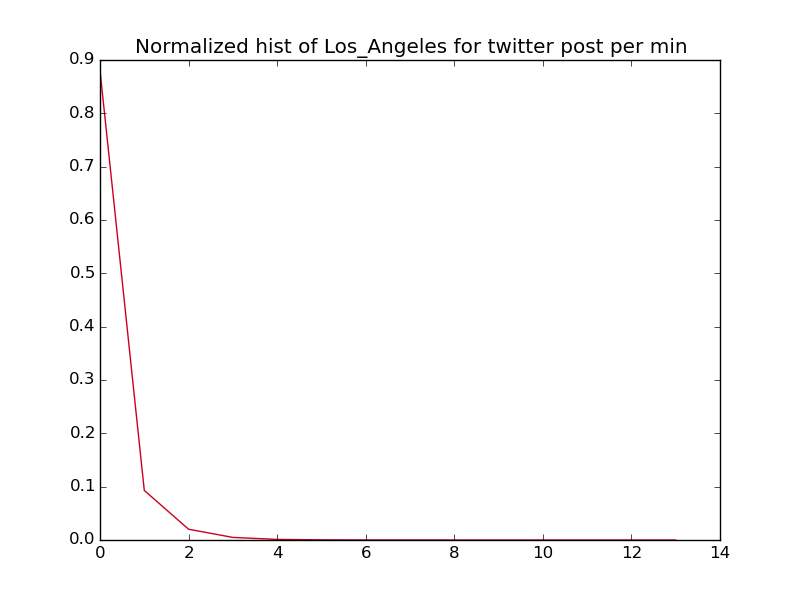
\includegraphics[scale=0.8]{Los_Angeleshisto.png}
\end{center}
\caption{Histogram of Los Angeles }
 \label {fig:2}
 \end{figure}
 
 \begin{figure}[H]
  \begin{center}
      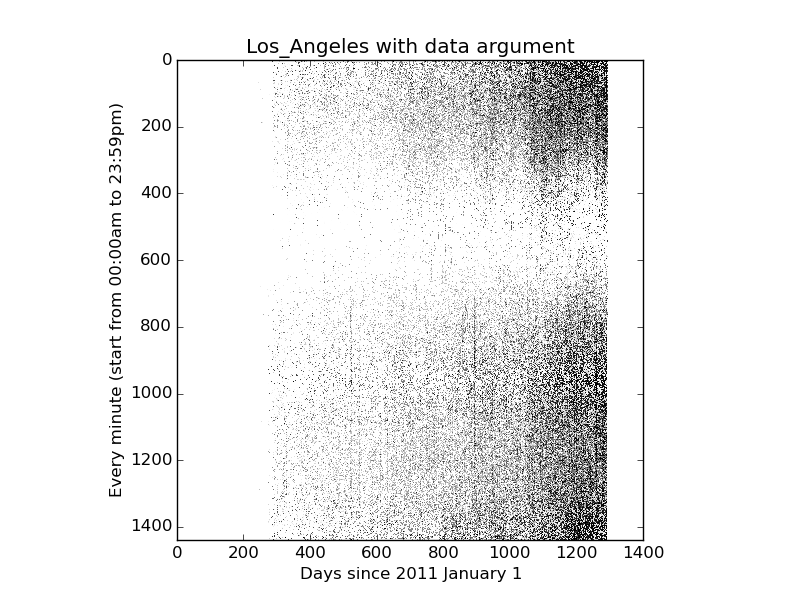
\includegraphics[scale=0.8]{Los_Angelesbinary.png}
\end{center}
\caption{Los Angeles every minute with data argumentation}
 \label {fig:2}
 \end{figure}



 \begin{figure}[H]
  \begin{center}
      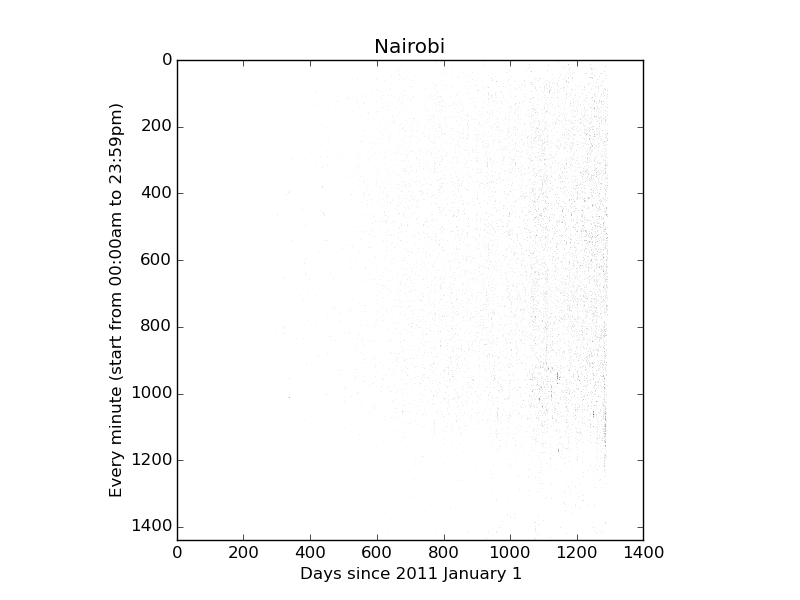
\includegraphics[scale=0.8]{Nairobi.png}
\end{center}
\caption{Nairobi every minute without data argumentation}
 \label {fig:2}
 \end{figure}
 
 
  \begin{figure}[H]
  \begin{center}
      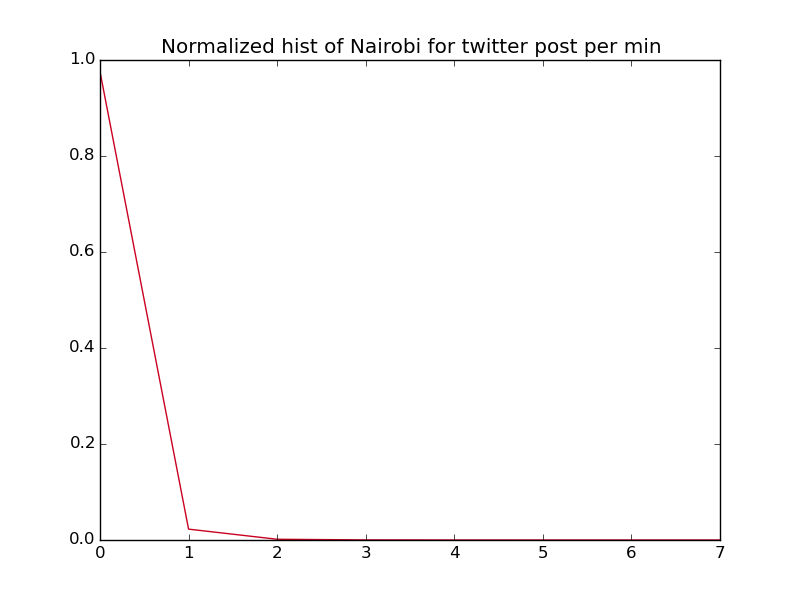
\includegraphics[scale=0.8]{Nairobihisto.png}
\end{center}
\caption{Histogram of Nairobi}
 \label {fig:2}
 \end{figure}
 
 
  \begin{figure}[H]
  \begin{center}
      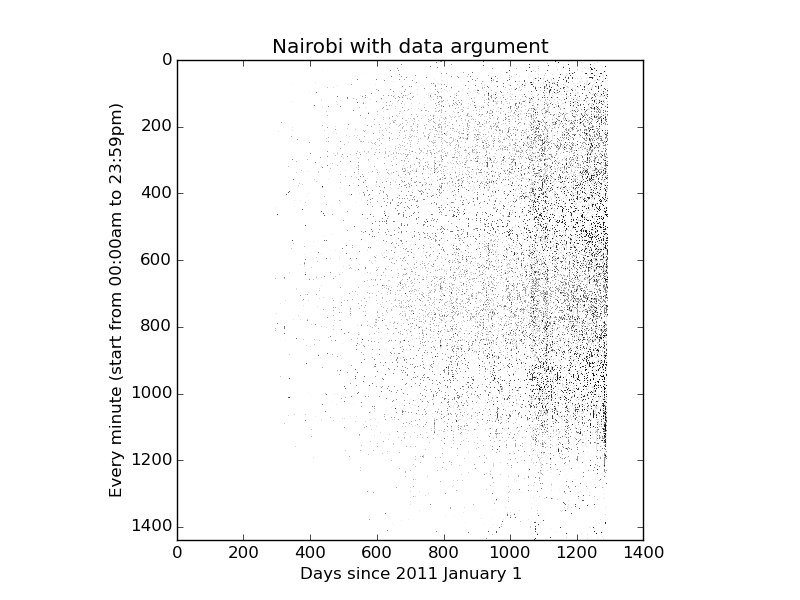
\includegraphics[scale=0.8]{Nairobibinary.png}
\end{center}
\caption{Nairobi every minute with data argumentation}
 \label {fig:2}
 \end{figure}
 
 


  \begin{figure}[H]
  \begin{center}
      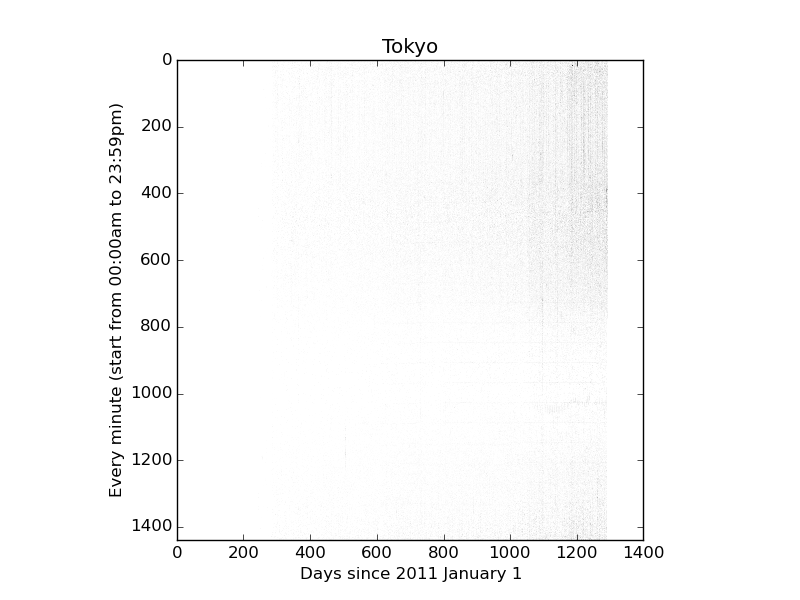
\includegraphics[scale=0.8]{Tokyo.png}
\end{center}
\caption{Tokyo every minute without data argumentation}
 \label {fig:2}
 \end{figure}
 
 
   \begin{figure}[H]
  \begin{center}
      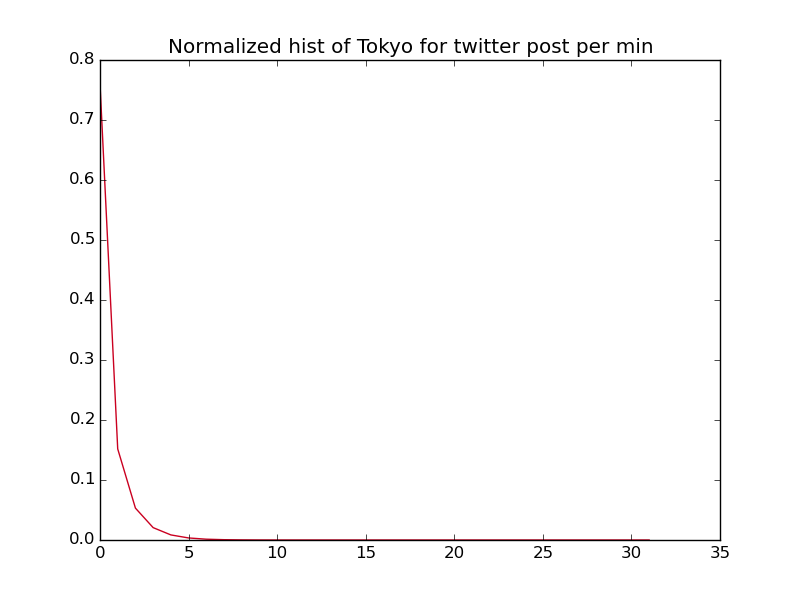
\includegraphics[scale=0.8]{Tokyohisto.png}
\end{center}
\caption{Histogram of Tokyo}
 \label {fig:2}
 \end{figure}
 
   \begin{figure}[H]
  \begin{center}
      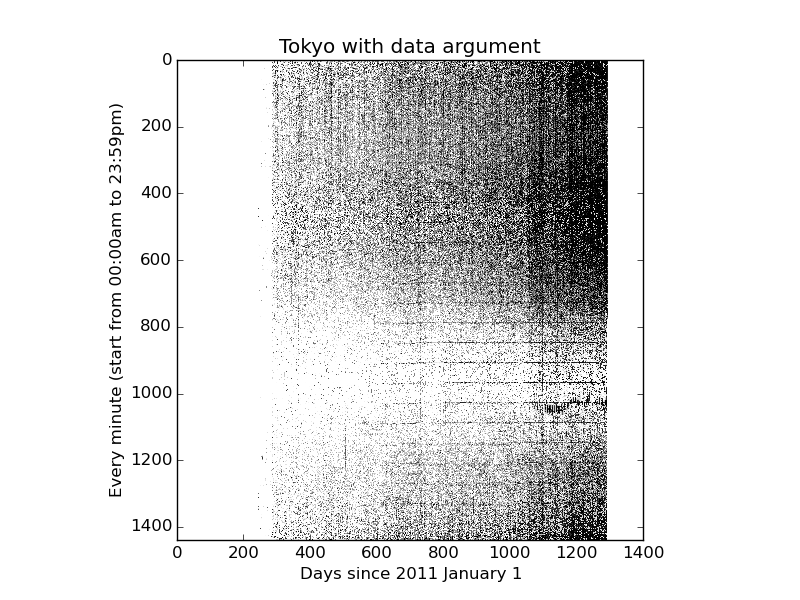
\includegraphics[scale=0.8]{Tokyobinary.png}
\end{center}
\caption{Tokyo every minute with data argumentation}
 \label {fig:2}
 \end{figure}
 
 \subsection{Observe the twitter post every 10 minutes}
 
 The observation results based on 30 minutes time slot are shown in this section. From the argumentation result we can see the pattern of each city is even more clear. It is not done yet. A further analysis is shown in the following section.\\
\begin{figure}[H]
  \begin{center}
      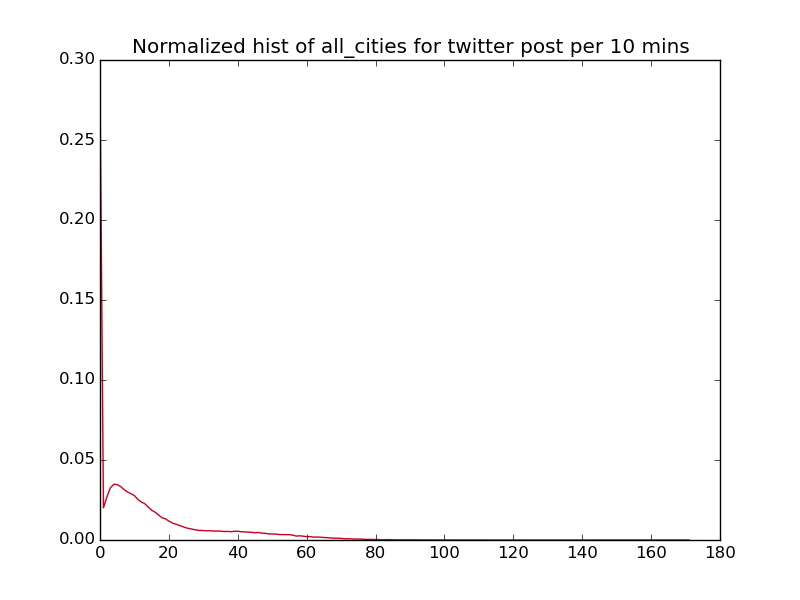
\includegraphics[scale=0.8]{1all_citieshisto.png}
\end{center}
\caption{Histogram of five cities when the observation time slot is every one minute}
 \label {fig:2}
 \end{figure}



\begin{figure}[H]
  \begin{center}
      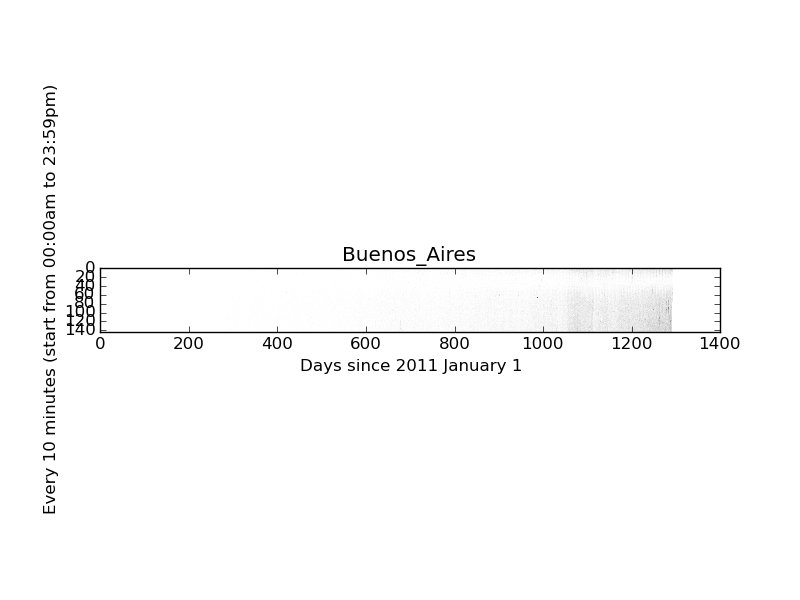
\includegraphics[scale=0.8]{1Buenos_Aires.png}
\end{center}
\caption{Buenos Aires every 10 minutes without data argumentation}
 \label {fig:2}
 \end{figure}



\begin{figure}[H]
  \begin{center}
      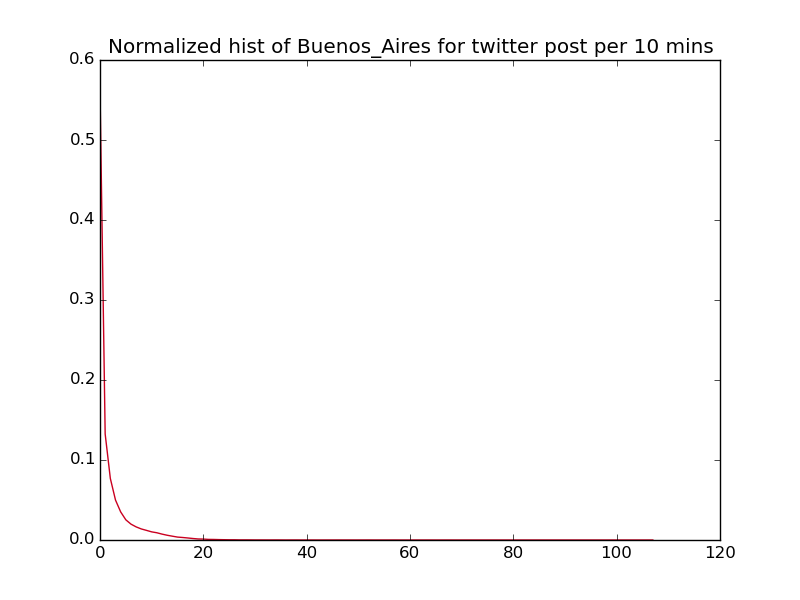
\includegraphics[scale=0.8]{1Buenos_Aireshisto.png}
\end{center}
\caption{Histogram of Buenos Aires}
 \label {fig:2}
 \end{figure}


\begin{figure}[H]
  \begin{center}
      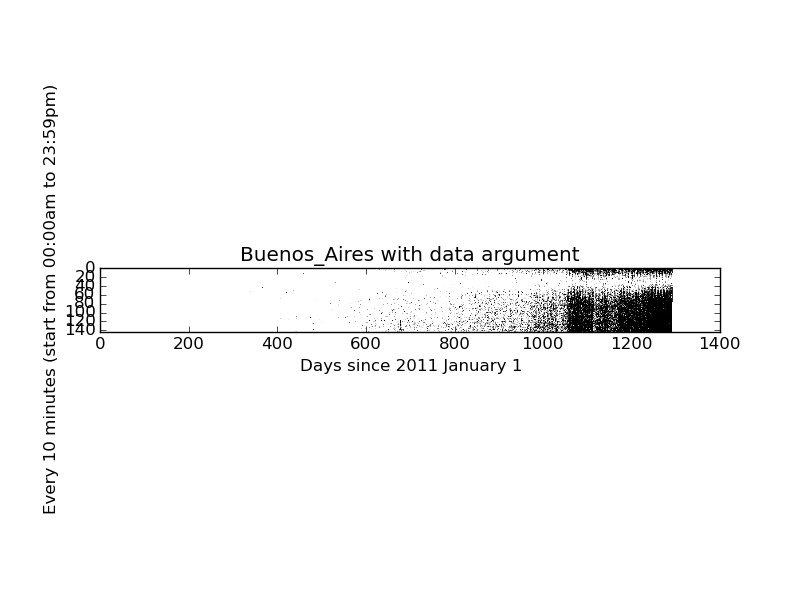
\includegraphics[scale=0.8]{1Buenos_Airesbinary.png}
\end{center}
\caption{Buenos Aires every 10 minutes with data argumentation}
 \label {fig:2}
 \end{figure}










\begin{figure}[H]
  \begin{center}
      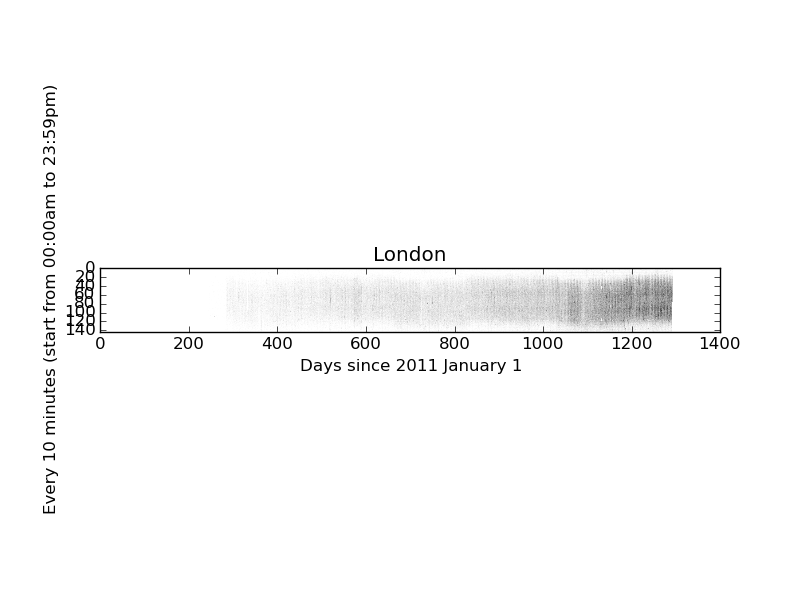
\includegraphics[scale=0.8]{1London.png}
\end{center}
\caption{London every 10 minutes without data argumentation}
 \label {fig:2}
 \end{figure}

\begin{figure}[H]
  \begin{center}
      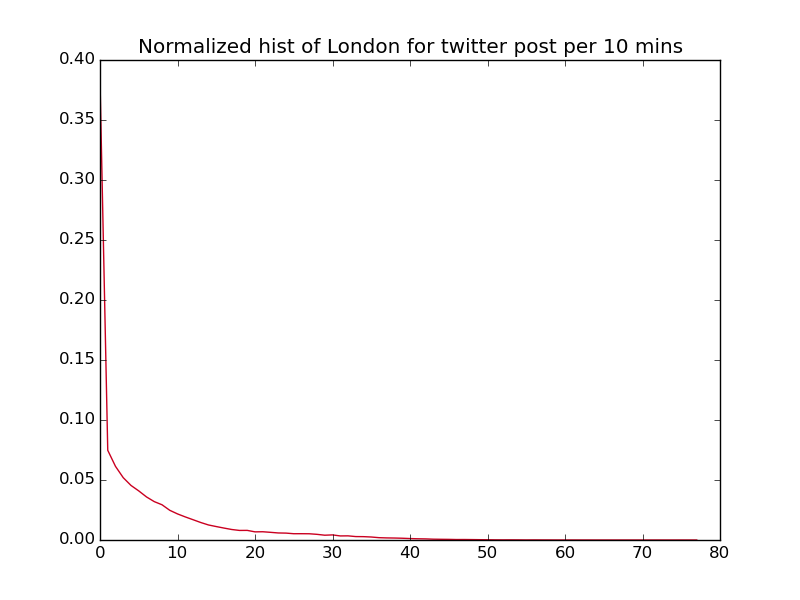
\includegraphics[scale=0.8]{1Londonhisto.png}
\end{center}
\caption{Histogram of London}
 \label {fig:2}
 \end{figure}

\begin{figure}[H]
  \begin{center}
      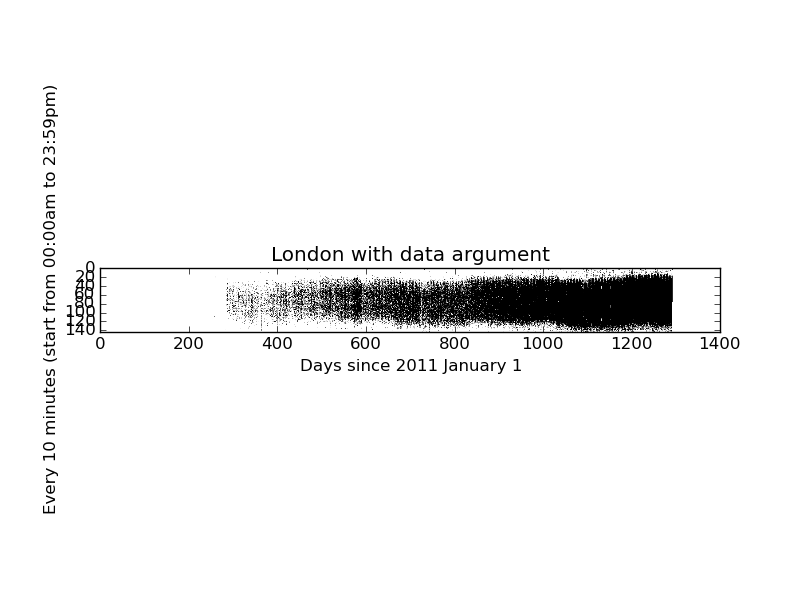
\includegraphics[scale=0.8]{1Londonbinary.png}
\end{center}
\caption{London every 10 minutes with data argumentation}
 \label {fig:2}
 \end{figure}






\begin{figure}[H]
  \begin{center}
      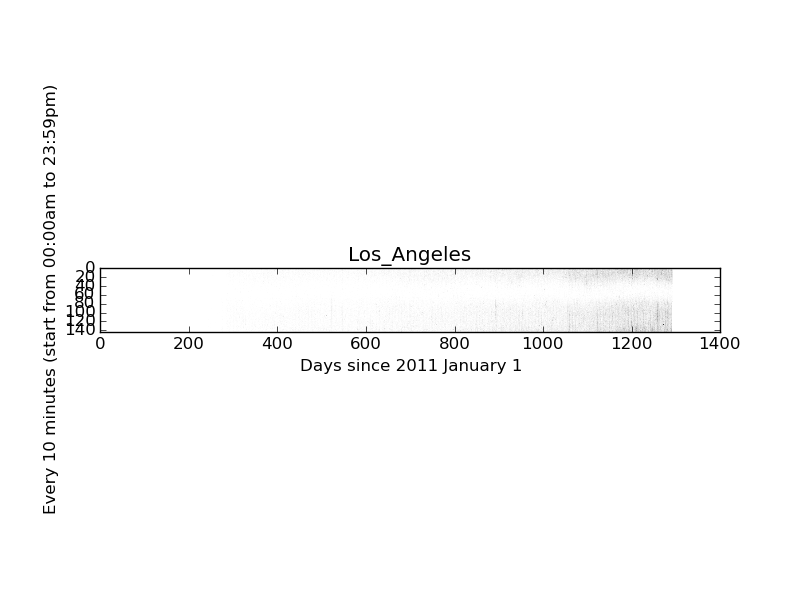
\includegraphics[scale=0.8]{1Los_Angeles.png}
\end{center}
\caption{Los Angeles every 10 minutes without data argumentation}
 \label {fig:2}
 \end{figure}
 
 \begin{figure}[H]
  \begin{center}
      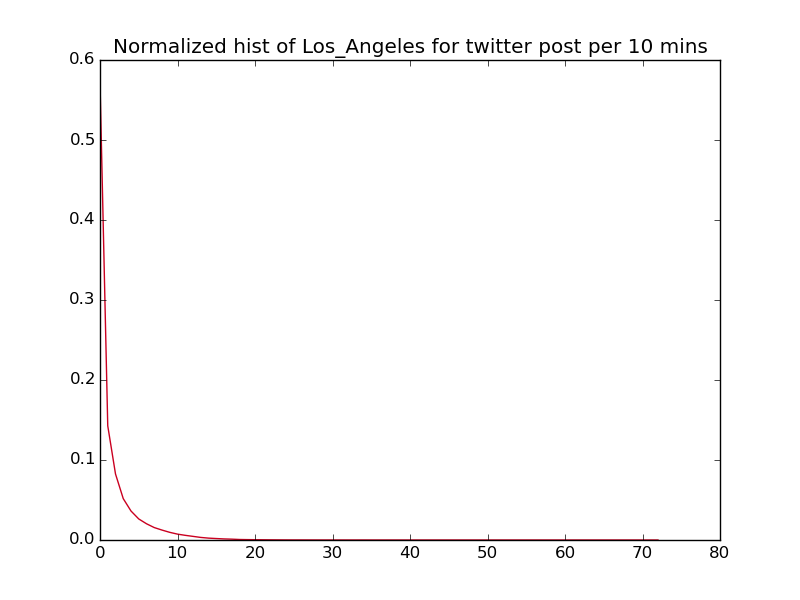
\includegraphics[scale=0.8]{1Los_Angeleshisto.png}
\end{center}
\caption{Histogram of Los Angeles }
 \label {fig:2}
 \end{figure}
 
 \begin{figure}[H]
  \begin{center}
      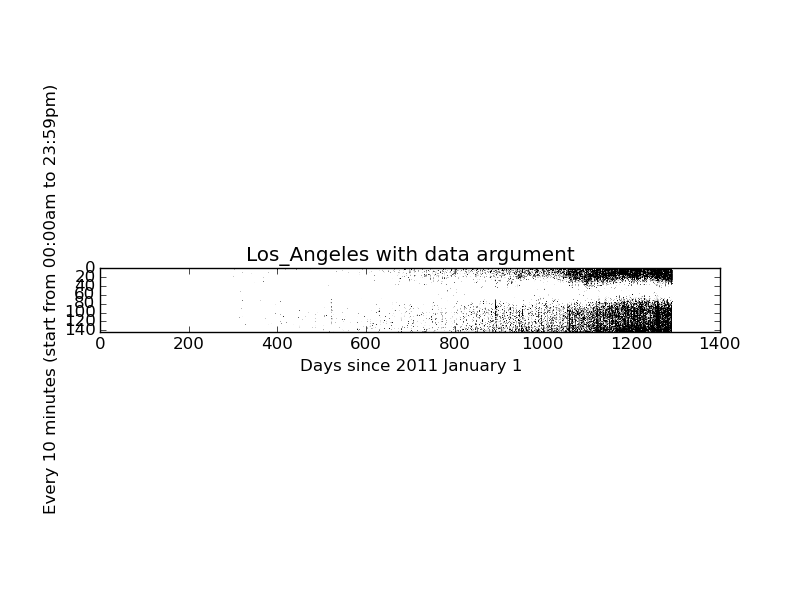
\includegraphics[scale=0.8]{1Los_Angelesbinary.png}
\end{center}
\caption{Los Angeles every 10 minutes with data argumentation}
 \label {fig:2}
 \end{figure}



 \begin{figure}[H]
  \begin{center}
      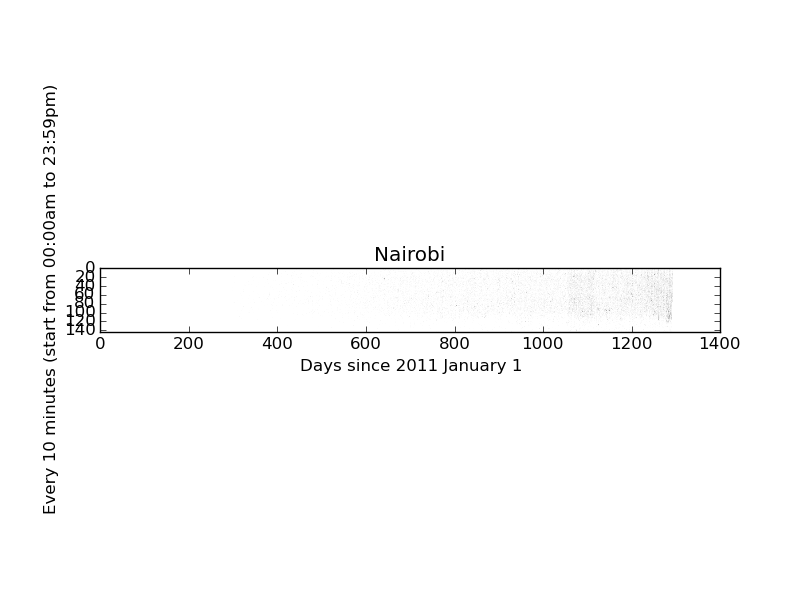
\includegraphics[scale=0.8]{1Nairobi.png}
\end{center}
\caption{Nairobi every 10 minutes without data argumentation}
 \label {fig:2}
 \end{figure}
 
 
  \begin{figure}[H]
  \begin{center}
      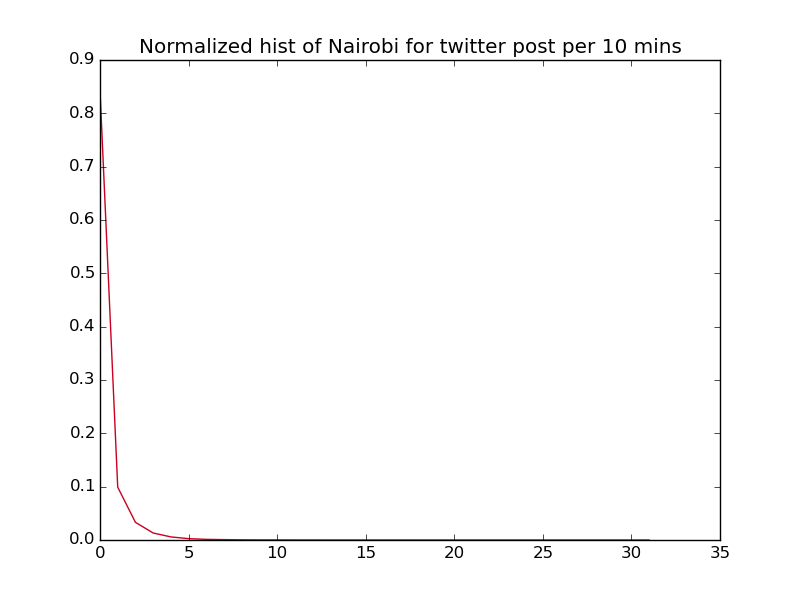
\includegraphics[scale=0.8]{1Nairobihisto.png}
\end{center}
\caption{Histogram of Nairobi}
 \label {fig:2}
 \end{figure}
 
 
  \begin{figure}[H]
  \begin{center}
      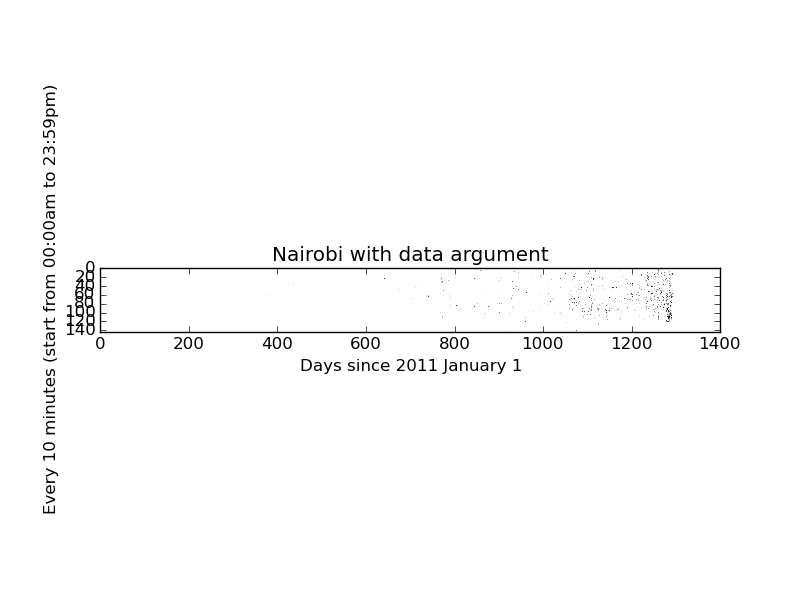
\includegraphics[scale=0.8]{1Nairobibinary.png}
\end{center}
\caption{Nairobi every 10 minutes with data argumentation}
 \label {fig:2}
 \end{figure}
 
 


  \begin{figure}[H]
  \begin{center}
      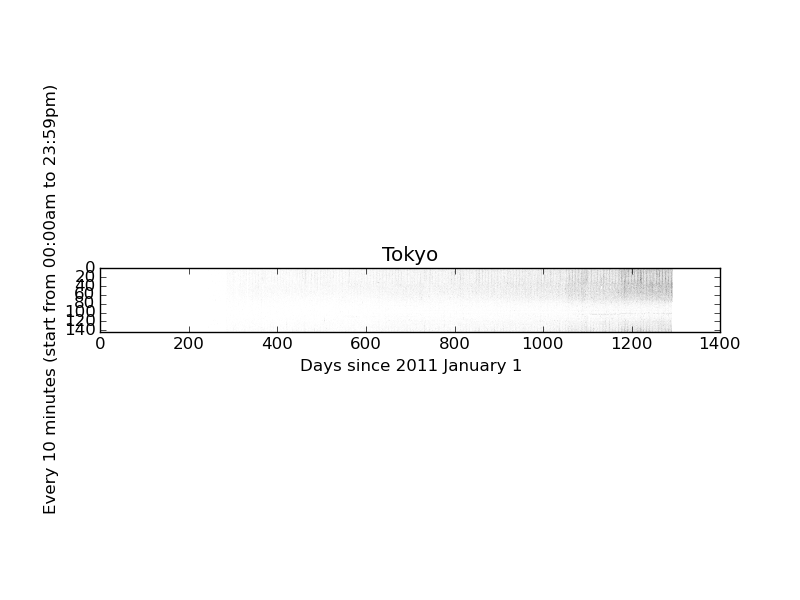
\includegraphics[scale=0.8]{1Tokyo.png}
\end{center}
\caption{Tokyo every 10 minutes without data argumentation}
 \label {fig:2}
 \end{figure}
 
 
   \begin{figure}[H]
  \begin{center}
      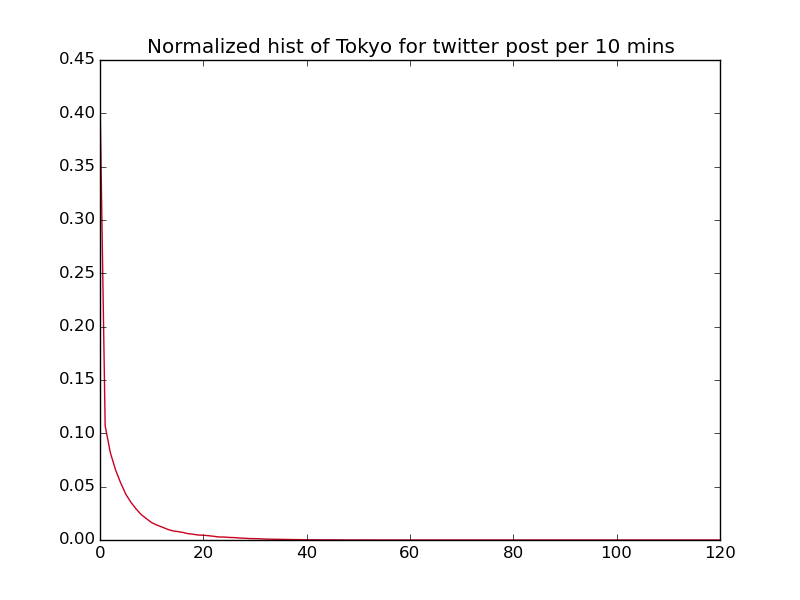
\includegraphics[scale=0.8]{1Tokyohisto.png}
\end{center}
\caption{Histogram of Tokyo}
 \label {fig:2}
 \end{figure}
 
   \begin{figure}[H]
  \begin{center}
      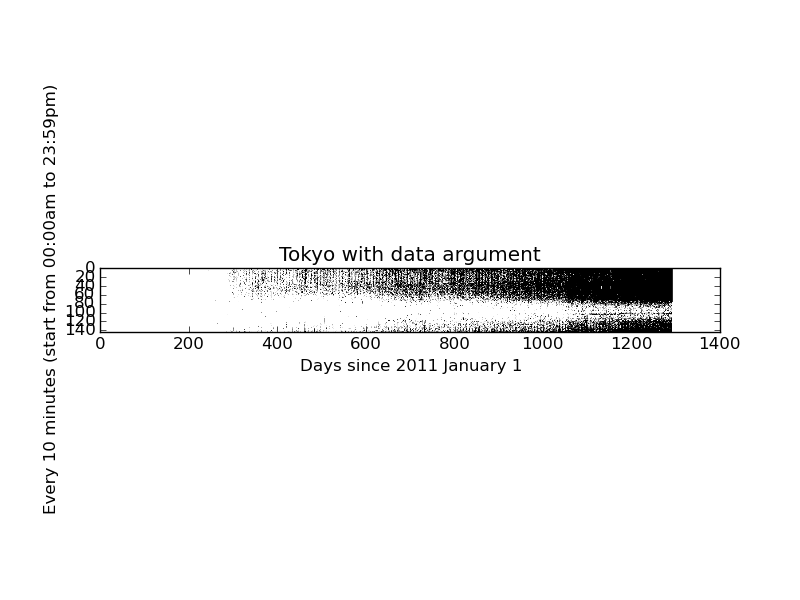
\includegraphics[scale=0.8]{1Tokyobinary.png}
\end{center}
\caption{Tokyo every 10 minutes with data argumentation}
 \label {fig:2}
 \end{figure}
 
 
  \subsection{Observe the activity level of a city based on the twitter post number every 10 minutes}
  
  The activity level is defined as: $twitter Post Number Per Time Slot /totalPostNumber4theWholeDay$ A specified threshold is chosen to do the data argumentation. The results are given in the following figures.\\
  
  From those results, we can see when the observations number becomes a large enough value, the status is more stable which can be well explained by the law of large number. Based on this, the last step will be done to get the sleeping time of a specified city which is doing the analysis based on the last 50 days data. The last 50 days data is more stable as the data size is big enough and also the activation model of a specified city will not be changed within 50 days. Then the data analysis based on the last 50 days generated the final result shown in figure 2. By this step, we can have a better understanding about  the sleeping time of a city.\\
  

\begin{figure}[H]
  \begin{center}
      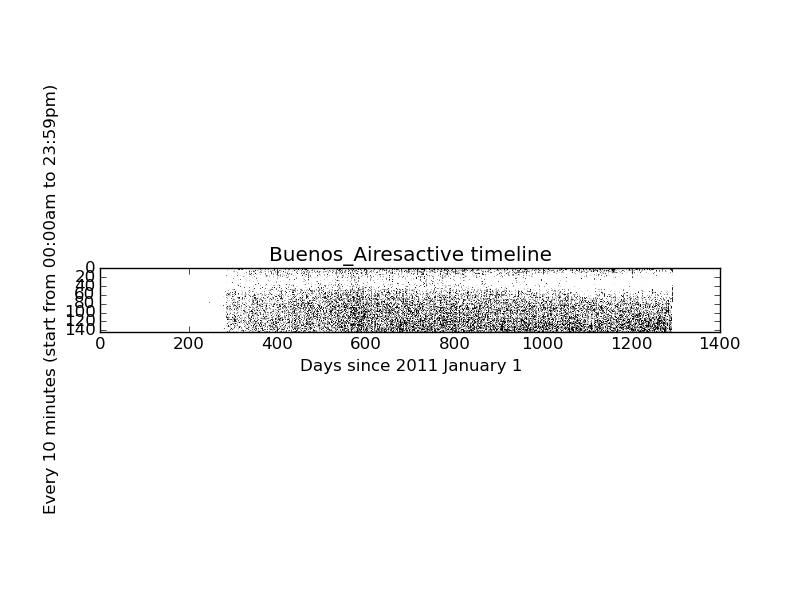
\includegraphics[scale=0.8]{Buenos_Airesbinary3.png}
\end{center}
\caption{Buenos Aires activation ratio based on every 10 minutes twitter post data  with data argumentation}
 \label {fig:2}
 \end{figure}




\begin{figure}[H]
  \begin{center}
      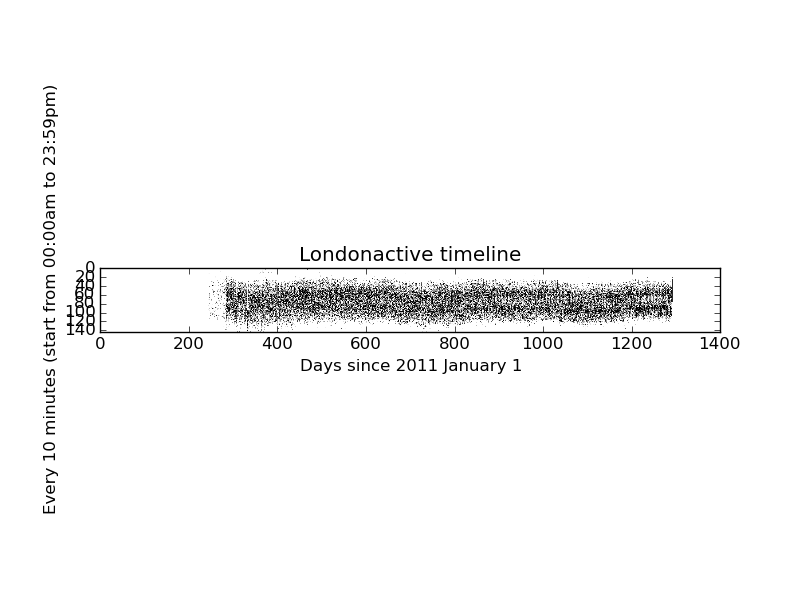
\includegraphics[scale=0.8]{Londonbinary3.png}
\end{center}
\caption{London activation ratio based on every 10 minutes twitter post data  with data argumentation}
 \label {fig:2}
 \end{figure}






 
 \begin{figure}[H]
  \begin{center}
      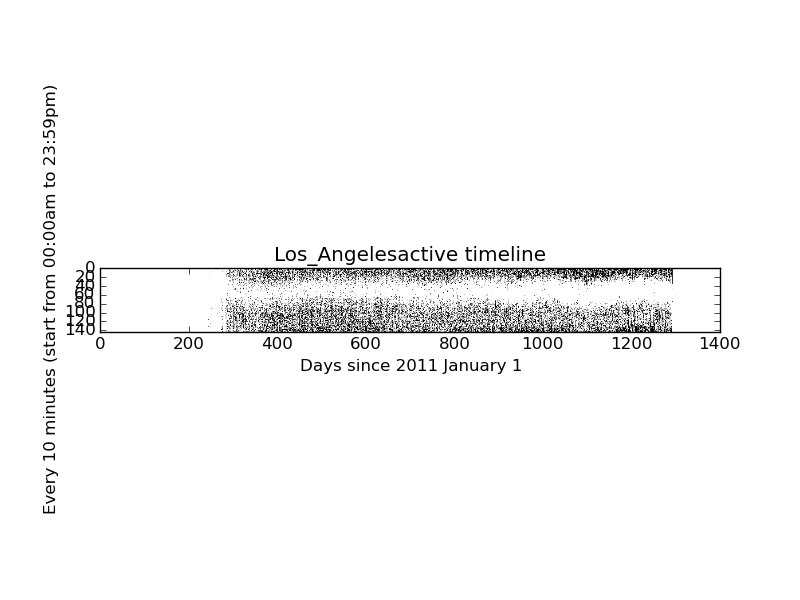
\includegraphics[scale=0.8]{Los_Angelesbinary3.png}
\end{center}
\caption{Los Angeles activation ratio based on every 10 minutes twitter post data  with data argumentation}
 \label {fig:2}
 \end{figure}




 

 
 
  \begin{figure}[H]
  \begin{center}
      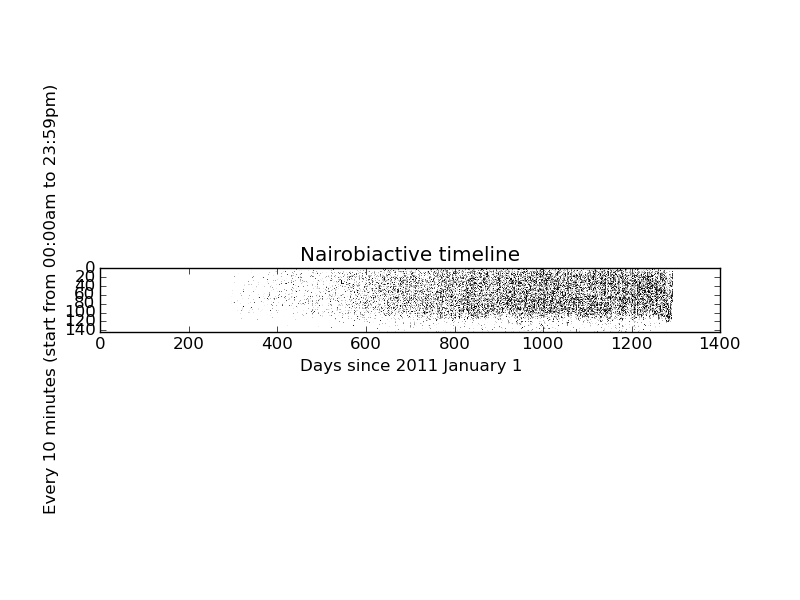
\includegraphics[scale=0.8]{Nairobibinary3.png}
\end{center}
\caption{Nairobi activation ratio based on every 10 minutes twitter post data  with data argumentation}
 \label {fig:2}
 \end{figure}
 
 

 
   \begin{figure}[H]
  \begin{center}
      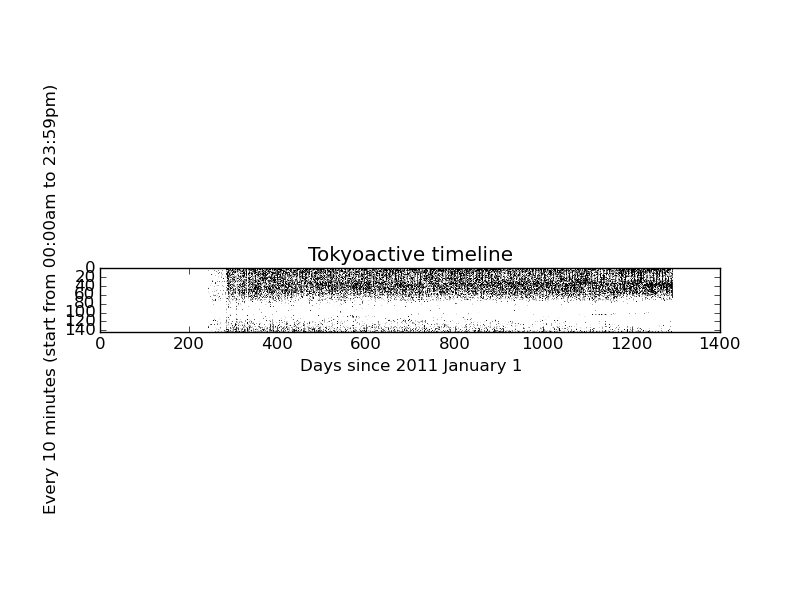
\includegraphics[scale=0.8]{Tokyobinary3.png}
\end{center}
\caption{Tokyo activation ratio based on every 10 minutes twitter post data  with data argumentation}
 \label {fig:2}
 \end{figure}
\section{Acknowledgement}

Thanks for professor Lev Manovich sharing the twitter data from the five cities. This article is part of course work of professor Lev Manovich's "Data Visualization" course at the Graduate Center, CUNY, during Spring 2017.  Thanks for Professor Lev Manovich's inspiration on building a good taste on data visualization such as how to choose the color, why does the detail of a good visualization arts matters and so on. Thanks again. As the twitter data belongs to professor Lev Manovich's Cultural Analytics Lab. This article will not be posted to public without the permission of the Cultural Analytics Lab.\\


 
  
 \end{document}